\chapter{Evaluation Fundamentals: From Loss to Sound Judgments}
\label{ch:evaluation}

\begin{keyinsight}
Evaluation is honest bookkeeping. When you measure a model's performance, you are measuring how efficiently it encodes information about your task. The numbers you report---loss, accuracy, calibration---are not arbitrary metrics. They are statements about compression, uncertainty, and decision quality. Understanding what each measurement means, and what it does not mean, is the difference between building systems that work and building systems that merely pass tests.
\end{keyinsight}

\vspace{1.5em}

We have spent the previous chapters building the foundations: information theory tells us that learning is compression, Bayesian inference tells us how to reason under uncertainty, and generalization theory tells us why models that compress well also predict well. Now we turn to a practical question that every builder of AI systems must answer: how do you know if your model is actually good?

\vspace{0.3cm}

This might seem like a simple question with obvious answers. You compute the loss on a test set. You measure accuracy. You run some benchmark. But each of these actions hides subtle choices, and those choices determine whether your evaluation tells you the truth or tells you what you want to hear. A model with low perplexity might generate incoherent text. A model with high accuracy might be poorly calibrated and dangerous to deploy. A model that dominates a benchmark might fail catastrophically on slightly different data.

\vspace{0.3cm}

This chapter teaches you how to evaluate models in a way that respects the information-theoretic foundations we have built. We will see that cross-entropy and perplexity measure average codelength, which is exactly what we want when compression is the goal, but they do not tell you whether the model's uncertainties are honest. We will explore calibration---the alignment between a model's confidence and its correctness---and learn simple techniques to diagnose and fix calibration failures. We will examine how sampling strategies like temperature and top-k change the distribution of outputs, and when each choice is appropriate. We will establish practical protocols for clean evaluation that avoid the traps of data contamination and train-test leakage. And finally, we will distill what you should report: a small, stable set of measurements that tell the truth about your model's capabilities and limitations.

\vspace{0.3cm}

What matters is not the number of metrics you compute, but whether those metrics measure what you actually care about. Evaluation is a conversation between the model and reality, mediated by the measurements you choose. This chapter teaches you to make that conversation honest.

\vspace{2em}

%==========================
\section{What Evaluation Really Measures}
%==========================

Let us start by clarifying what we mean when we "evaluate" a model. At the most basic level, evaluation is measurement. You present the model with inputs, observe its outputs, and compute numbers that summarize its performance. But what do those numbers measure, and what do they miss?

\vspace{1em}

\subsection{Cross-Entropy and Perplexity: Average Codelength}

We introduced cross-entropy in Chapter 1 as the expected codelength when you use distribution $q$ to encode data from distribution $p$. For a language model evaluated on a test set, cross-entropy tells you how many nats (or bits) the model needs, on average, to encode each token in the test set. Lower cross-entropy means better compression, which means the model has learned patterns that apply to new data.

\vspace{0.3cm}

Perplexity is the exponential of cross-entropy, and it gives an intuitive sense of the model's uncertainty. A perplexity of twelve means the model has the same average uncertainty as if it were uniformly choosing among twelve options at each prediction, though in reality the model's uncertainty varies from nearly certain to highly confused, with twelve being the geometric mean.

\vspace{0.3cm}

Here is what cross-entropy and perplexity tell you well: they measure the average quality of the model's probability distribution over the data. If you care about compression, density estimation, or general-purpose predictive accuracy, these metrics are exactly right. A model with lower test perplexity has learned the test distribution better than a model with higher perplexity. This is a crisp, information-theoretic statement.

\vspace{0.3cm}

But here is what they do not tell you. Cross-entropy averages over all predictions, treating easy and hard examples equally (weighted by frequency). It does not distinguish between a model that is confidently wrong and one that is cautiously uncertain. It does not tell you whether the model's probabilities are calibrated. It does not measure worst-case performance or robustness to distribution shift. And for generative tasks where you sample rather than compute likelihoods, cross-entropy measures the quality of the distribution, not the quality of samples from that distribution.

\vspace{1.5em}

\begin{examplebox}
\textbf{When Lower Loss Does Not Mean Better}

\vspace{0.5em}

Suppose you train two language models on the same dataset and evaluate them on a held-out test set. Model A achieves a test perplexity of ten. Model B achieves a test perplexity of twelve. By the cross-entropy criterion, Model A is better---it compresses the test data more efficiently.

\vspace{0.5em}

But now you use these models to generate text by sampling. You notice that Model A often produces fluent but factually incorrect statements, while Model B hedges more, using phrases like "it is possible that" or "some sources suggest." When you measure factual accuracy on a question-answering task, Model B outperforms Model A.

\vspace{0.5em}

What happened? Model A learned to assign high probability to common but sometimes incorrect patterns. It memorized correlations in the training data that do not reflect ground truth. Its perplexity is low because it confidently predicts what a typical training example would say, not what is true. Model B, by contrast, spreads probability more cautiously, which increases its perplexity but also makes it less likely to confidently assert falsehoods.

\vspace{0.5em}

The lesson: lower perplexity measures better compression of the test distribution, but if that distribution contains systematic errors or biases, better compression can mean worse behavior for downstream tasks. You must evaluate what you care about, not just what is easy to measure.
\end{examplebox}

\vspace{1.5em}

\subsection{The Gap Between Loss and Decisions}

Cross-entropy is a loss function---it tells you how to score the model's predictions. But in practice, you rarely care about loss in isolation. You care about decisions made using the model's predictions. A medical diagnosis system does not just output probabilities; it makes recommendations that affect treatment. A content moderation system does not just score toxicity; it decides what to remove.

\vspace{0.3cm}

The connection between loss and decision quality depends on the decision problem and on whether the probabilities you use are trustworthy. In the ideal case---when the model's predicted probabilities match the true conditional probabilities for the outcomes you care about---minimizing expected loss under those probabilities is equivalent to minimizing expected cost under the true distribution. But if the model is overconfident, you will make too many aggressive decisions. If it is underconfident, you will be too cautious.

\vspace{0.3cm}

This is where evaluation must go beyond aggregate loss. You need to check whether the model's uncertainty estimates are honest. You need to measure performance on the specific decisions you care about, not just the average prediction quality. And you need to test robustness: does the model fail gracefully when inputs shift away from the training distribution, or does it confidently produce nonsense?

\vspace{0.3cm}

From Chapter 2, we know that different loss functions lead to different optimal decisions. Zero-one loss favors the mode of the predictive distribution. Squared loss favors the mean. Log loss (cross-entropy) favors the full distribution. If your evaluation metric does not align with your deployment loss, you are optimizing the wrong thing. A model with the lowest cross-entropy might not have the highest accuracy if accuracy is what you deploy on.

\vspace{1em}

\subsection{Why Benchmarks Lie (Sometimes)}

Benchmarks are designed to make evaluation easy and reproducible. They provide a fixed test set, a standardized metric, and a leaderboard that lets you compare models. This is valuable, but benchmarks have failure modes that you must understand.

\vspace{0.3cm}

First, benchmarks can saturate. When many models achieve near-perfect scores, the benchmark stops discriminating between good models and great ones. The gap between ninety-eight percent accuracy and ninety-nine percent accuracy might be meaningless if both models fail on the same hard cases that are underrepresented in the test set.

\vspace{0.3cm}

Second, benchmarks can be gamed. If the test set is public, or if practitioners have implicit knowledge of it through repeated evaluation, models can overfit to the benchmark without generalizing more broadly. This is called "adaptive overfitting," and it is insidious because it does not show up in your training-test split---the test set itself becomes contaminated by implicit feedback.

\vspace{0.3cm}

Third, benchmarks measure what is easy to measure, not necessarily what matters. Natural language understanding is hard to formalize, so benchmarks use proxies like multiple-choice questions or textual entailment. But these proxies do not capture the full range of skills required for real-world understanding. A model can excel at multiple-choice questions while failing at open-ended reasoning or factual accuracy.

\vspace{0.3cm}

The solution is not to abandon benchmarks but to use them carefully. Treat benchmark scores as lower bounds on capability, not as complete descriptions of model quality. Complement benchmark evaluation with task-specific tests, adversarial examples, and human evaluation on cases that matter for your application. And when reporting results, be transparent about what the benchmark measures and what it does not.

\vspace{2em}

%==========================
\section{Uncertainty and Calibration: The Essentials}
%==========================

A well-calibrated model is one whose confidence matches its correctness. If the model assigns ninety percent probability to an event, that event should happen ninety percent of the time. If the model says it is uncertain, it should actually be uncertain. Calibration is the bridge between loss (which measures average performance) and trust (which requires honest uncertainty).

\vspace{1em}

\subsection{Confidence Versus Correctness}

Let us make the distinction precise. Confidence is what the model reports: the probability it assigns to its prediction. Correctness is ground truth: whether the prediction matches reality. In a $K$-class classifier, a common definition of confidence is the probability assigned to the predicted class (the max-softmax). In a language model, at each step it is the probability assigned to the next token you choose or sample. For a well-calibrated model, confidence and correctness align. For a poorly calibrated model, they diverge.

\vspace{0.3cm}

Consider a binary classifier that outputs probabilities. For all examples where the model predicts positive with confidence between ninety and one hundred percent, the true positive rate should be close to the model's average confidence in that bin (for example, around ninety-five percent if the average confidence is ninety-five percent). For examples where the model predicts positive with confidence between fifty and sixty percent, the true positive rate should similarly match the bin's average confidence (around fifty-five percent if that is what the model reports). This alignment is calibration.

\vspace{0.3cm}

Why does calibration matter? Because downstream decisions depend on probabilities being honest. If a model says there is a ten percent chance of a rare disease, a doctor might order further tests but not immediate treatment. If the true rate is actually thirty percent when the model says ten percent, the doctor's decision will be wrong. Calibration failures cause misaligned decisions.

\vspace{0.3cm}

For language models and other generative models, calibration becomes more subtle. You can measure calibration at the token level (does the model's predicted probability for each token match the frequency with which that token appears next in the evaluation data?) or at the sequence level (does the model's overall confidence in a generated sequence match the quality of that sequence?). Token-level calibration is easier to measure but does not guarantee good sequence-level behavior, because errors can compound across a sequence.

\vspace{1em}

\subsection{Reliability Diagrams: Visualizing Calibration}

The standard tool for diagnosing calibration is the reliability diagram, also called a calibration plot. Here is how you construct one. You bin your predictions by confidence: all predictions with confidence between zero and ten percent, ten to twenty percent, and so on up to ninety to one hundred percent. For each bin, you compute the average predicted confidence and the actual frequency of the predicted event. You then plot these as points: the $x$-axis is the average confidence, the $y$-axis is the actual frequency.

\vspace{0.3cm}

For a perfectly calibrated model, all points lie on the diagonal line $y = x$. If points lie above the diagonal, the model is underconfident: it predicts lower probabilities than the true frequencies. If points lie below the diagonal, the model is overconfident: it predicts higher probabilities than the true frequencies.

\vspace{0.3cm}

Modern neural networks, especially large ones, tend to be overconfident. They assign very high probabilities to predictions that are only moderately likely to be correct. This overconfidence comes from the optimization process: models are trained to maximize likelihood, which rewards assigning high probability to the training data. There is no explicit penalty for being overconfident on examples the model has not seen.

\vspace{0.3cm}

Reliability diagrams are simple but powerful. They immediately reveal whether your model's probabilities are trustworthy. If you see systematic deviation from the diagonal, you know you have a calibration problem, and you need to fix it before deploying the model for decision-making.

\vspace{1em}

\begin{figure}[t]
\centering
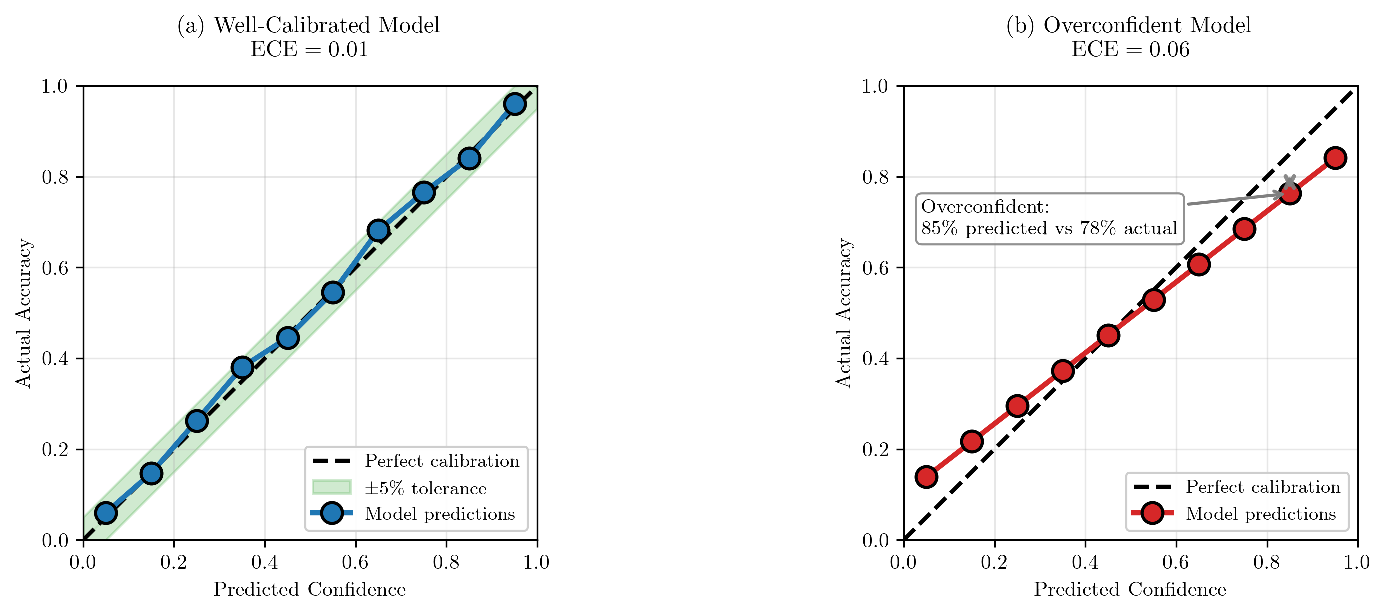
\includegraphics[width=\linewidth]{code/figures/ch10_calibration/fig_10_1_reliability_diagram.pdf}
\caption{Reliability diagrams bin predictions by confidence and compare expected confidence to empirical accuracy; deviations from the diagonal expose over- or underconfidence.}
\label{fig:reliability_diagram}
\end{figure}

\vspace{1em}

\subsection{Temperature Scaling: A Simple Fix}

Temperature scaling is the simplest and most effective method for post-hoc calibration. The idea is to add a temperature parameter $T$ that rescales the logits (pre-softmax activations) before converting them to probabilities. For a classifier with logits $z_1, \ldots, z_K$, the calibrated probabilities are:

\vspace{0.3cm}

\begin{equation}
p_i = \frac{\exp(z_i / T)}{\sum_{j=1}^K \exp(z_j / T)}
\end{equation}

\vspace{0.3cm}

When $T = 1$, you get the original probabilities. When $T > 1$, the distribution is "softened"---probabilities become more uniform, reducing overconfidence. When $T < 1$, the distribution is "sharpened"---probabilities become more peaked, increasing confidence. The optimal temperature is found by minimizing the negative log-likelihood on a held-out calibration set.

\vspace{0.3cm}

Why does this work? Temperature scaling preserves the ranking of probabilities---it does not change which class has the highest probability, so it does not affect top-one accuracy. But it changes the magnitude of the probabilities, which affects calibration. By choosing $T$ to minimize negative log-likelihood on a validation set, you correct for the model's systematic bias toward over- or underconfidence, and calibration metrics like ECE typically improve as a result.

\vspace{0.3cm}

Temperature scaling has limitations. It is a single global parameter, so it cannot fix calibration issues that vary across different regions of the input space. If the model is overconfident on some types of examples and underconfident on others, a single temperature cannot correct both. More sophisticated methods like Platt scaling or isotonic regression can handle non-uniform calibration errors, but they require more data and are more prone to overfitting.

\vspace{1.5em}

\begin{figure}[t]
\centering
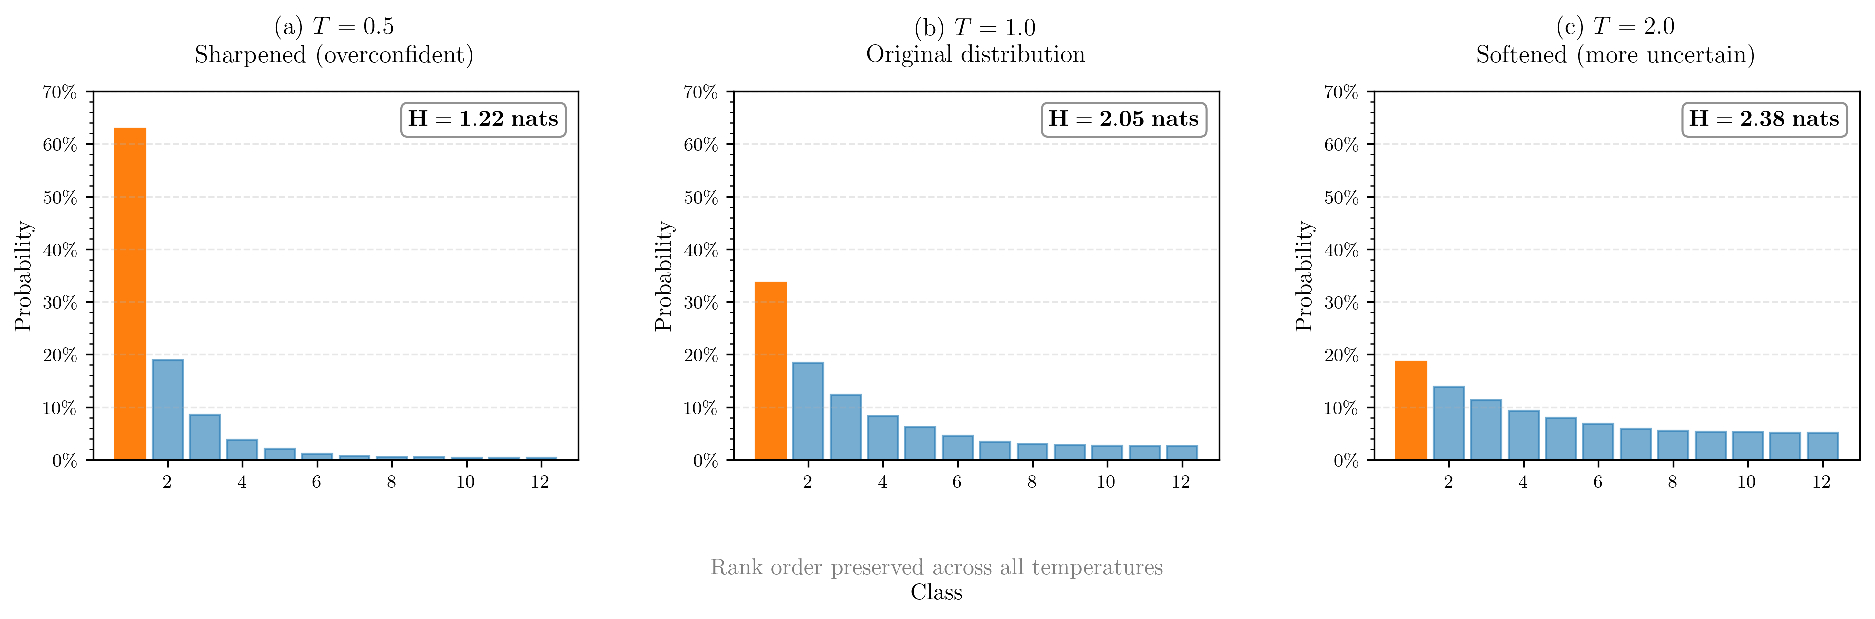
\includegraphics[width=\linewidth]{code/figures/ch10_calibration/fig_10_2_temperature_scaling.pdf}
\caption{Temperature scaling rescales logits with a single parameter $T$, softening or sharpening the predicted distribution without changing argmax decisions.}
\label{fig:temperature_scaling}
\end{figure}

\vspace{1.5em}

\begin{examplebox}
\textbf{Calibrating a Classifier with Temperature Scaling}

\vspace{0.5em}

Suppose you have trained an image classifier on ImageNet and you evaluate it on a held-out validation set of ten thousand images. You compute the predicted probabilities and construct a reliability diagram. You observe that predictions with average confidence around ninety percent have actual accuracy around seventy percent---the model is overconfident.

\vspace{0.5em}

You apply temperature scaling. You try values of $T$ from $0.5$ to $3.0$ in increments of $0.1$, computing the negative log-likelihood on the validation set for each value. You find that $T = 1.5$ gives the lowest validation loss.

\vspace{0.5em}

With $T = 1.5$, you recompute the calibrated probabilities and construct a new reliability diagram. The points now lie much closer to the diagonal. Predictions with average confidence around sixty percent (after rescaling with $T = 1.5$) have actual accuracy around sixty percent. The model is calibrated.

\vspace{0.5em}

Importantly, the top-one accuracy has not changed---temperature scaling does not affect which class has the highest probability, so the model still makes the same predictions when you take the argmax. But the probabilities themselves are now honest, which means you can use them for decision-making with proper expected utility calculations.
\end{examplebox}

\vspace{1.5em}

\begin{figure}[t]
\centering
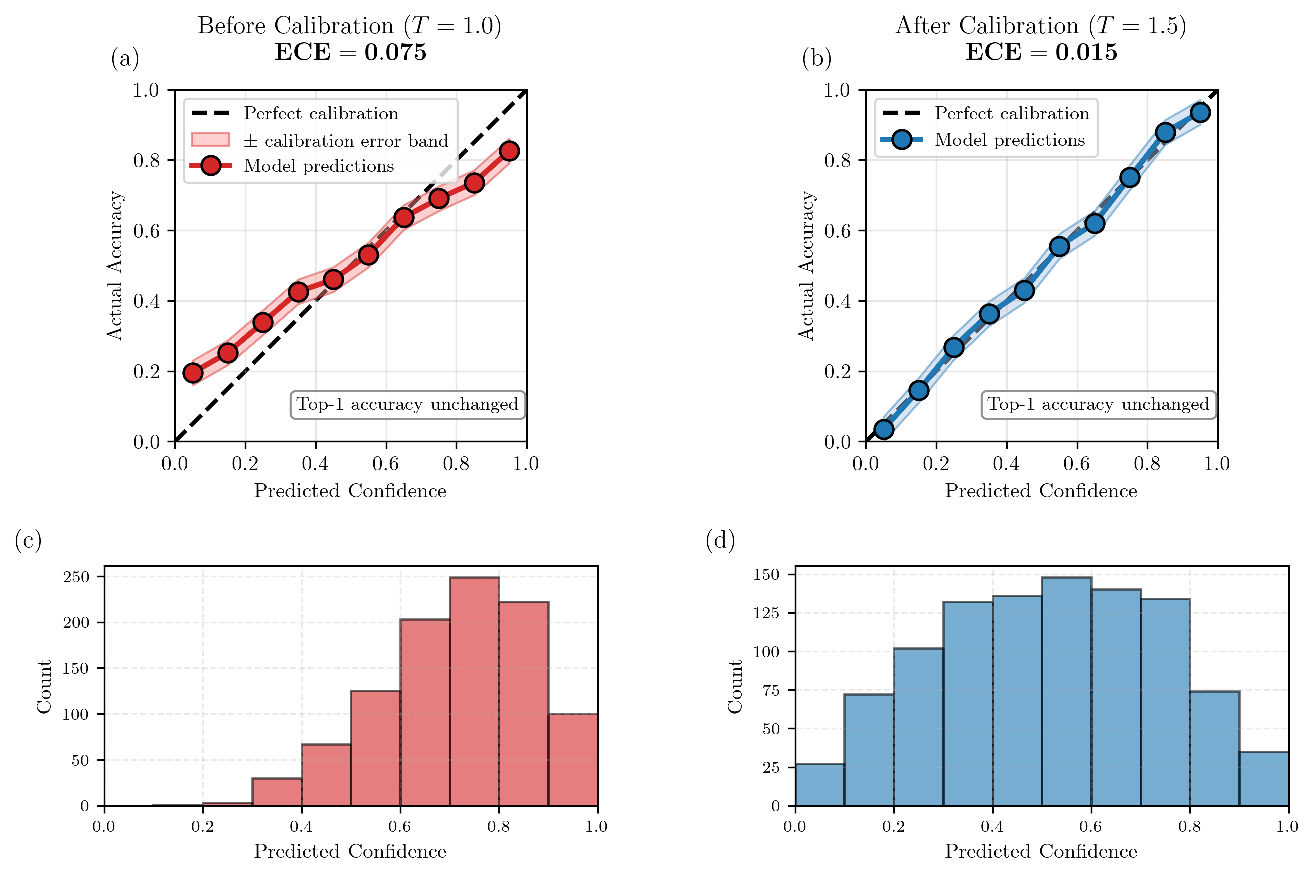
\includegraphics[width=\linewidth]{code/figures/ch10_calibration/fig_10_5_before_after_calibration.pdf}
\caption{Post-hoc calibration (e.g., temperature scaling) moves an overconfident model toward the diagonal reliability line, reducing Expected Calibration Error.}
\label{fig:calibration_before_after}
\end{figure}

\vspace{1.5em}

\subsection{Token-Level Versus Sequence-Level Calibration}

For language models, calibration has two distinct flavors. Token-level calibration asks: when the model assigns probability $p$ to a particular next token, does that token actually appear next with frequency $p$ in the evaluation data? (This is a statement about the data distribution, not a claim that there is a single semantically "correct" continuation.) Sequence-level calibration asks: when the model generates a complete sequence with some overall confidence score, does that score correlate with the quality of the sequence?

\vspace{0.3cm}

Token-level calibration is easier to measure because you can evaluate it on every token prediction in your test set. You bin predictions by the model's assigned probability, and you check whether the empirical frequency of that token occurring matches the predicted probability. If the model is well-calibrated at the token level, its per-token surprisals are honest.

\vspace{0.3cm}

Sequence-level calibration is harder because you need to define what "quality" means for a generated sequence. For tasks with a single correct answer (like translation or summarization with a reference), you can measure whether sequences the model assigns high probability to are actually good according to some metric. For open-ended generation, you might need human evaluation to judge quality, and you can check whether the model's confidence (perhaps measured by the average token probability or some aggregate score) correlates with human judgments.

\vspace{0.3cm}

Token-level calibration does not guarantee sequence-level calibration. Even if each token's probability is honest, errors can compound. A model might assign fifty percent probability to each of ten independent binary choices in a sequence. The probability of getting all ten correct is less than one in a thousand, but the model's per-token calibration would look fine. This compounding is why sequence-level evaluation matters for generative tasks, even when token-level metrics look good.

\vspace{0.3cm}

In practice, you should measure both. Token-level calibration tells you whether the model's basic probability estimates are trustworthy. Sequence-level calibration tells you whether those estimates compose in a way that produces reliable overall confidence. If token-level calibration is poor, fix it first with temperature scaling. If sequence-level calibration is poor even when token-level is good, you might need to aggregate uncertainties differently or use techniques like conformal prediction, which we will discuss later.

\vspace{2em}

\begin{figure}[t]
\centering
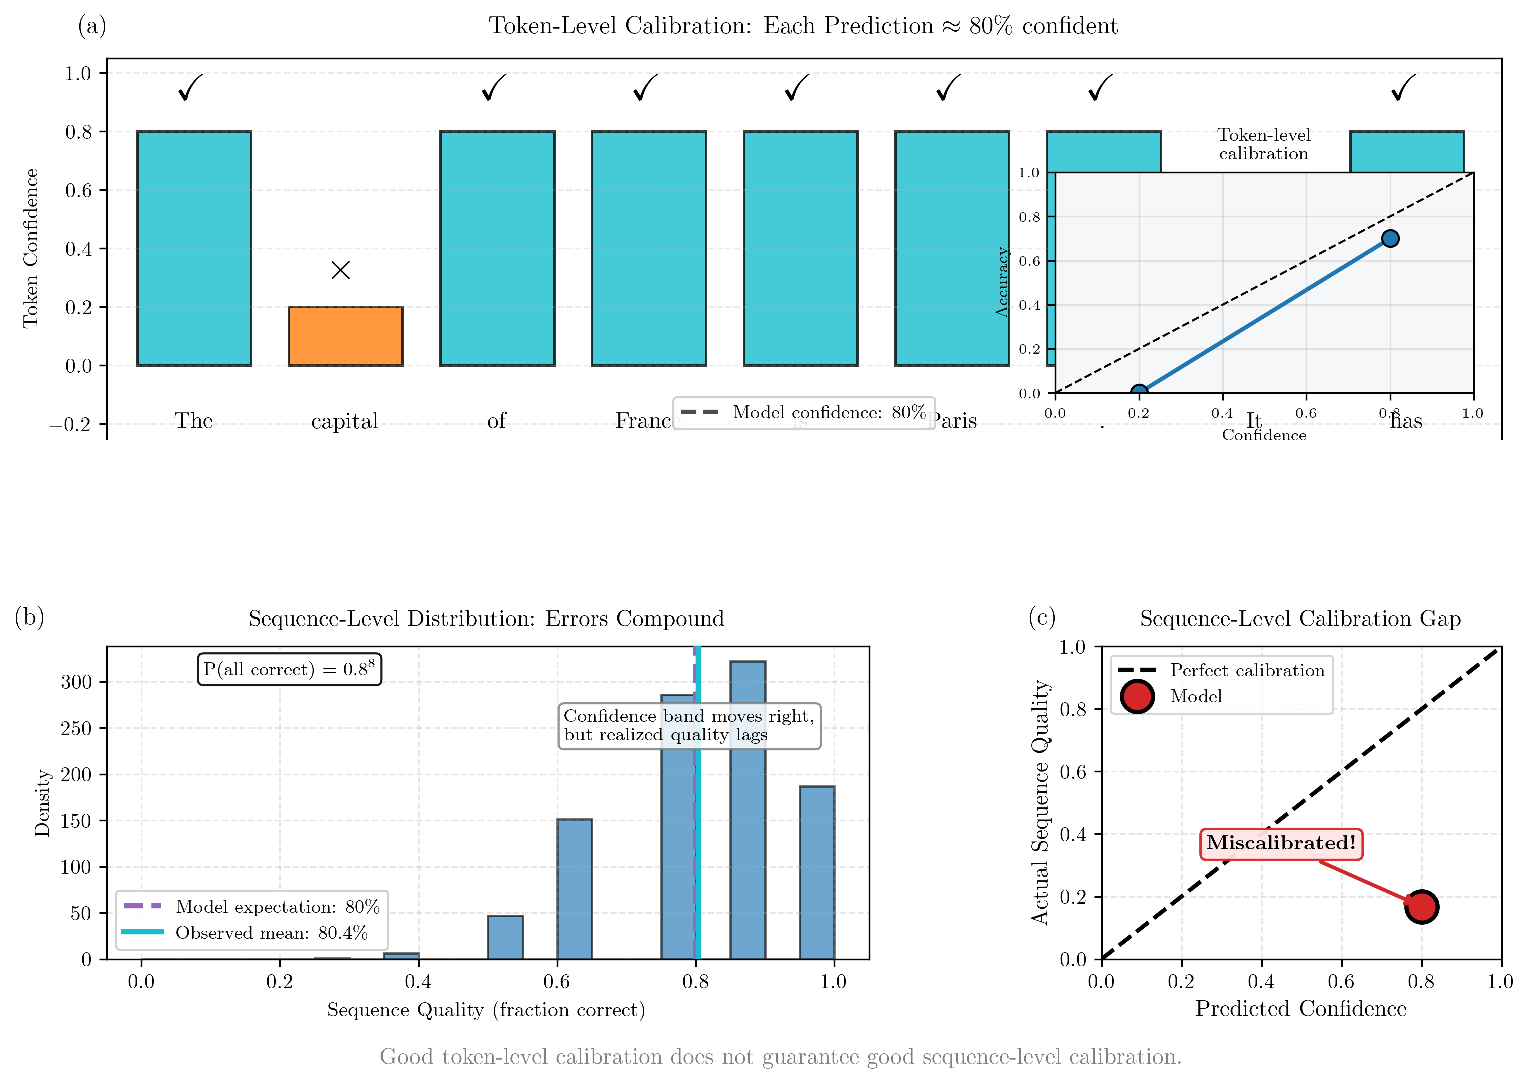
\includegraphics[width=\linewidth]{code/figures/ch10_calibration/fig_10_6_token_vs_sequence.pdf}
\caption{Token-level calibration may look perfect while sequence-level confidence remains misaligned; evaluate both to understand deployment risk.}
\label{fig:token_vs_sequence_calibration}
\end{figure}

\vspace{2em}

%==========================
\section{Sampling as a Decision Dial}
%==========================

When you use a generative model, you usually do not compute likelihoods---you sample. The model defines a distribution over sequences, and you draw samples from that distribution to produce outputs. But there is not a unique way to sample. You can adjust the "randomness" of the sampling process, and these adjustments change the diversity, quality, and error rates of the outputs in predictable ways.

\vspace{1em}

\subsection{Temperature: Controlling Entropy}

Temperature is the same parameter we just saw for calibration, but in the sampling context, it serves a different purpose. When you sample from a language model, you typically apply a temperature to the logits before sampling. The temperature controls the entropy of the distribution: higher temperature makes the distribution more uniform (more exploratory, more diverse outputs), lower temperature makes it more peaked (more conservative, more likely to repeat high-probability sequences).

\vspace{0.3cm}

At $T = 1$, you sample from the model's original distribution. At $T \to \infty$, all tokens become equally likely---you sample uniformly at random. At $T \to 0$, you take the argmax---you deterministically choose the highest-probability token at each step, which is equivalent to greedy decoding.

\vspace{0.3cm}

The choice of temperature is a tradeoff. Lower temperature gives you more consistent, "safer" outputs that stick close to high-probability regions of the model's distribution. This reduces the chance of nonsensical or off-topic generations, but it also makes the outputs less diverse and more repetitive. Higher temperature increases diversity and can produce more creative or surprising outputs, but it also increases the probability of errors, contradictions, and low-quality samples.

\vspace{0.3cm}

There is no universally correct temperature. The right choice depends on your task and your tolerance for errors. For tasks where correctness is critical---like generating code or answering factual questions---you want low temperature to minimize errors. For tasks where diversity is valuable---like creative writing or brainstorming---you want higher temperature to explore more possibilities. For most tasks, $T \in [0.7, 1.0]$ works well, but you should tune it empirically.

\vspace{1em}

\subsection{Top-$k$ and Nucleus Sampling: Truncating the Tail}

Temperature affects the entire distribution, but sometimes you want more control over which tokens are even considered. Top-$k$ sampling and nucleus sampling (also called top-$p$ sampling) are two methods that truncate the distribution before sampling, removing low-probability tokens from consideration.

\vspace{0.3cm}

Top-$k$ sampling works as follows. At each decoding step, you rank all tokens by their probability under the model. You keep only the top $k$ tokens, set the probabilities of all other tokens to zero, and renormalize the remaining probabilities to sum to one. Then you sample from this truncated distribution. Common choices for $k$ are between ten and one hundred.

\vspace{0.3cm}

The advantage of top-$k$ is that it prevents the model from sampling extremely low-probability tokens that are likely to be errors or nonsense. The disadvantage is that $k$ is a fixed number, so it does not adapt to the model's uncertainty. When the model is very confident (most probability mass on a few tokens), keeping ten tokens might include some that have negligible probability. When the model is very uncertain (probability mass spread across many tokens), keeping only ten might exclude reasonable options.

\vspace{0.3cm}

Nucleus sampling addresses this by using a dynamic cutoff. Instead of keeping a fixed number of tokens, you keep the smallest set of tokens whose cumulative probability reaches a threshold $p$ (typically $p = 0.9$ or $p = 0.95$). This adapts to the model's confidence: when the model is certain, the nucleus is small; when it is uncertain, the nucleus is large.

\vspace{0.3cm}

Nucleus sampling tends to give more coherent outputs than top-$k$ because it avoids sampling from the long tail of low-probability tokens while still allowing the model to be diverse when the distribution is naturally flat. The choice of $p$ controls the tradeoff: higher $p$ includes more tokens and increases diversity; lower $p$ is more conservative and reduces errors. In practice, $p = 0.9$ or $p = 0.95$ works well for most generation tasks.

\vspace{1.5em}

\begin{examplebox}
\textbf{Comparing Sampling Strategies on a Simple Task}

\vspace{0.5em}

Suppose you prompt a language model to complete the sentence: "The capital of France is\_\_." The model assigns probabilities as follows: "Paris" (ninety-one percent), "paris" (three percent, lowercase variant), "Lyon" (two percent), "Marseille" (one percent), and other tokens share the remaining three percent across hundreds of possibilities.

\vspace{0.5em}

\textbf{Greedy decoding} ($T = 0$): Always outputs "Paris." Correct every time, but no diversity.

\vspace{0.5em}

\textbf{Temperature} $T = 1$: Samples from the full distribution. Ninety-one percent of the time you get "Paris," three percent "paris," occasionally you get other cities. Mostly correct, some variation.

\vspace{0.5em}

\textbf{Temperature} $T = 2$: Softens the distribution. "Paris" drops to maybe seventy percent, other options increase. More diversity, more errors.

\vspace{0.5em}

\textbf{Top-$k$ with $k = 5$}: Keeps "Paris," "paris," "Lyon," "Marseille," and maybe one other token. Renormalizes and samples. Almost always correct (Paris or paris), occasionally gets a wrong city. Prevents sampling from the long tail of nonsense tokens.

\vspace{0.5em}

\textbf{Nucleus with $p = 0.95$}: Keeps "Paris," "paris," and "Lyon" (cumulative probability ninety-six percent). Slightly more conservative than top-$k = 5$. Very rarely samples "Lyon," almost always correct.

\vspace{0.5em}

For this task, all methods work well because the model is very confident. The differences become more important when the model is uncertain or when you generate longer sequences where errors can compound.
\end{examplebox}

\vspace{1.5em}

\begin{figure}[t]
\centering
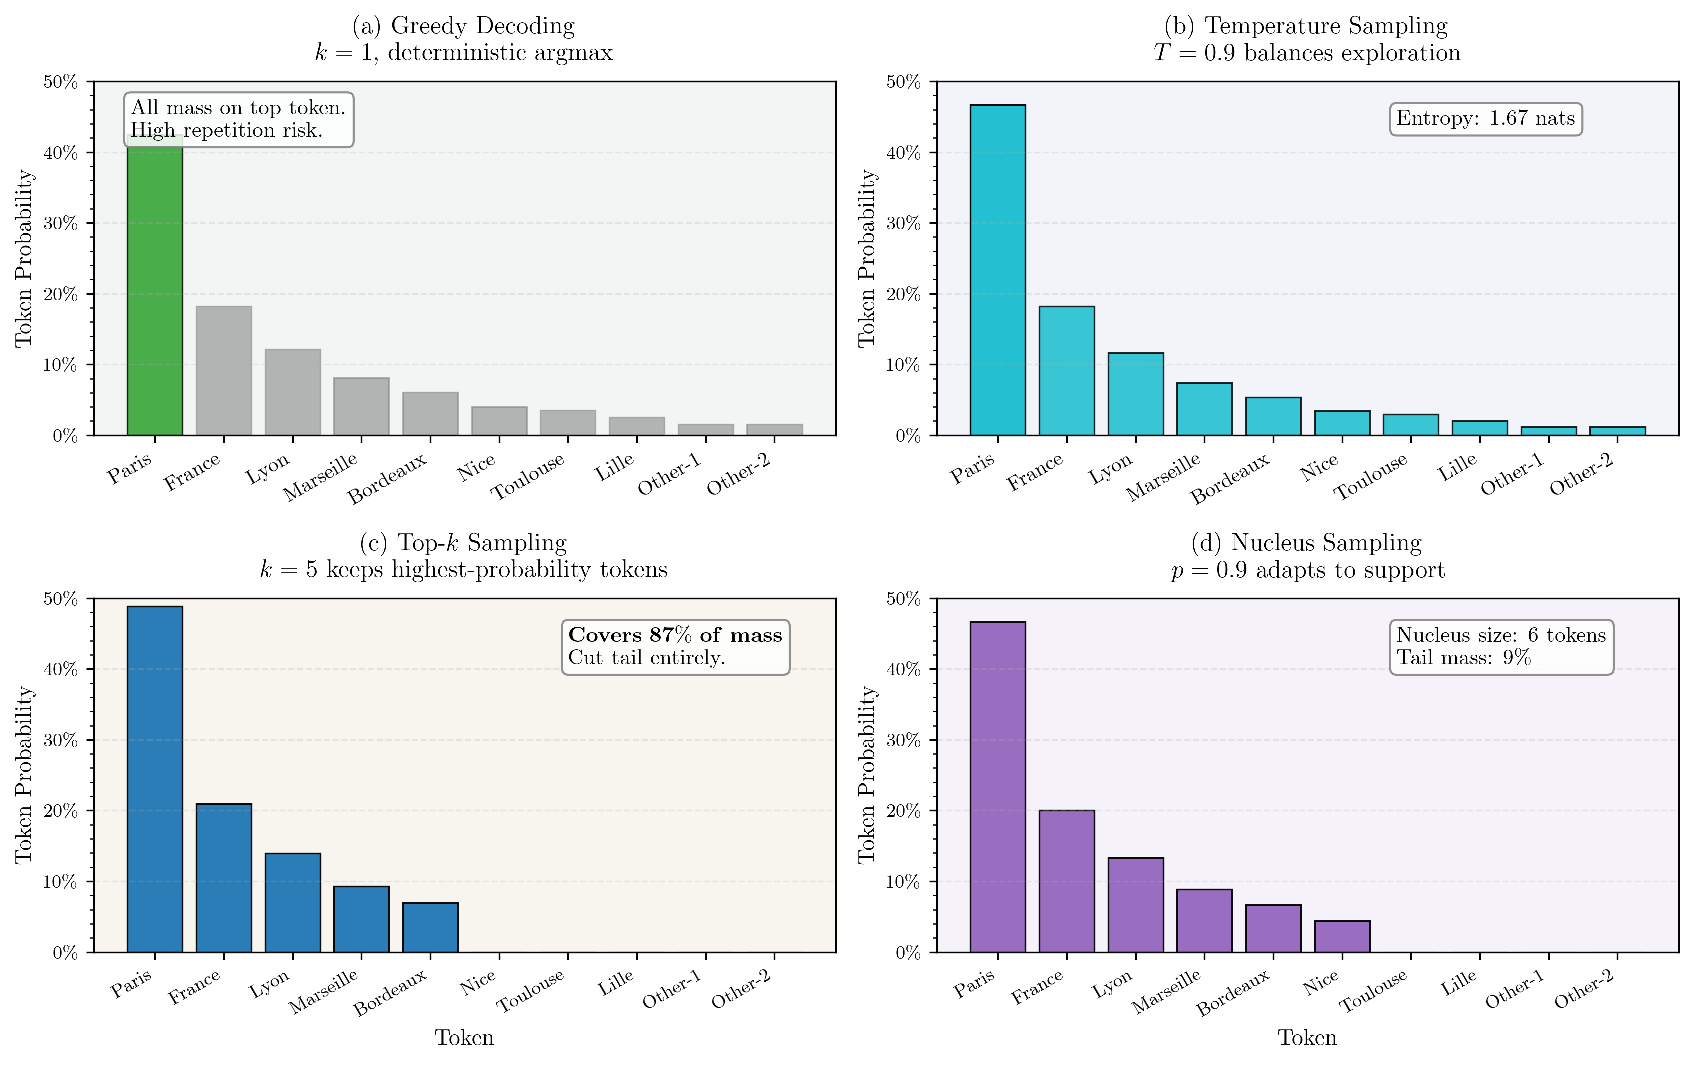
\includegraphics[width=\linewidth]{code/figures/ch10_calibration/fig_10_3_decoding_strategies.pdf}
\caption{Decoding strategies reshape the distribution: temperature rescales probabilities, top-$k$ truncates to a fixed set, and nucleus sampling adapts to cumulative mass.}
\label{fig:sampling_strategies}
\end{figure}

\vspace{1.5em}

\subsection{The Diversity-Error Tradeoff}

There is a fundamental tradeoff between diversity and error rate in sampling. If you want perfectly correct outputs, you should use greedy decoding (or very low temperature), but you will get repetitive, predictable results. If you want diverse, creative outputs, you should use high temperature or broad nucleus sampling, but you will get more errors, inconsistencies, and occasionally nonsensical generations.

\vspace{0.3cm}

This tradeoff is not a failing of the sampling methods---it is a reflection of the model's uncertainty. When the model is uncertain about what comes next, there genuinely are multiple plausible continuations. Sampling randomly captures this diversity. But some of those plausible continuations are wrong, and sampling randomly means you sometimes choose them.

\vspace{0.3cm}

The right point on this tradeoff depends on your application. For a chatbot, some errors are acceptable if the responses are more varied and interesting. For a medical diagnosis system, errors are unacceptable, so you should be very conservative. For creative writing assistance, diversity is the goal, so errors in the sense of "not the most probable continuation" are actually desirable---you want the model to explore less obvious possibilities.

\vspace{0.3cm}

You can visualize this tradeoff by running simple experiments. Generate many samples at different temperatures or with different nucleus thresholds. Measure both diversity (perhaps by counting unique sequences or measuring entropy of the sampled distribution) and error rate (perhaps by checking factual accuracy or coherence). Plot these against each other. You will see the tradeoff clearly: as you increase diversity, errors increase. The curve tells you where on the tradeoff your application should operate.

\vspace{1em}

\begin{figure}[t]
\centering
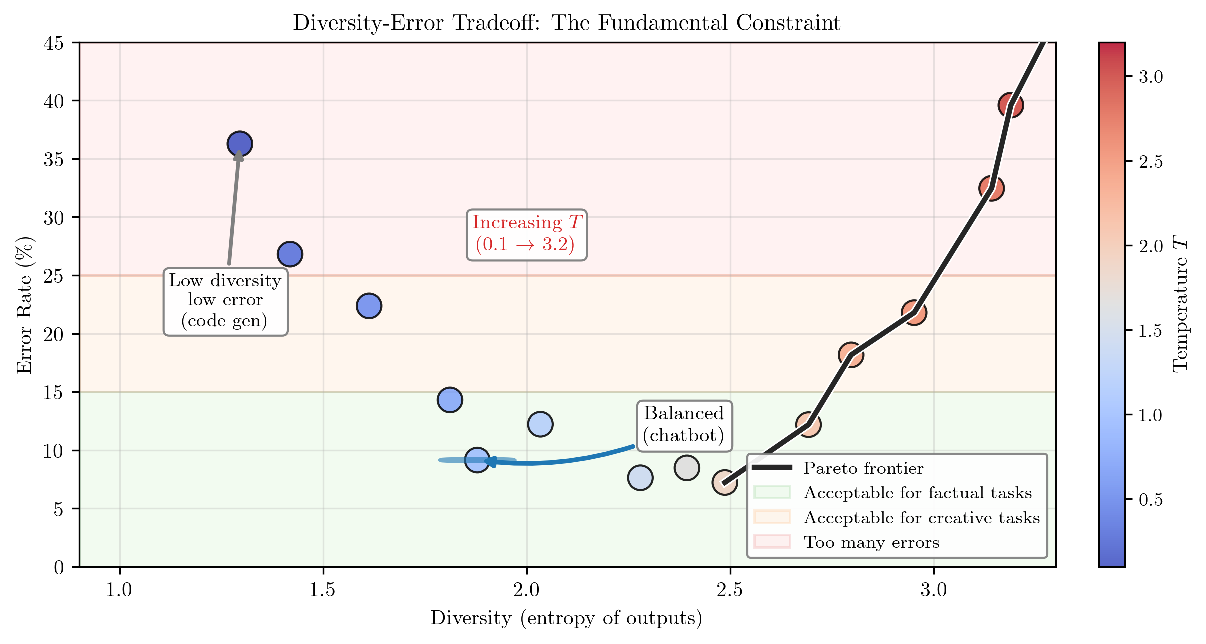
\includegraphics[width=\linewidth]{code/figures/ch10_calibration/fig_10_4_diversity_error_tradeoff.pdf}
\caption{Increasing randomness (temperature or nucleus mass) boosts diversity but also raises error rates; choose an operating point that matches application tolerance.}
\label{fig:diversity_error_tradeoff}
\end{figure}

\vspace{1em}

\subsection{When to Use Which Strategy}

Here is practical guidance for choosing a sampling strategy:

\vspace{0.3cm}

Use greedy decoding or very low temperature ($T < 0.3$) when correctness is critical and diversity is not important. Examples: generating code, answering factual questions, translating technical documents.

\vspace{0.3cm}

Use moderate temperature ($T \in [0.7, 1.0]$) with nucleus sampling ($p = 0.9$) for general-purpose generation where you want a balance of quality and diversity. Examples: chatbots, creative writing assistance, general question answering.

\vspace{0.3cm}

Use higher temperature ($T \in [1.0, 1.5]$) with nucleus sampling ($p = 0.95$) when you want to explore diverse possibilities and are willing to accept occasional errors. Examples: brainstorming, generating multiple candidate responses to choose from, creative tasks.

\vspace{0.3cm}

Use top-$k$ sampling with small $k$ (like ten to twenty) when you want to prevent the model from sampling extremely unlikely tokens but you do not want the adaptive behavior of nucleus sampling. This is less common in practice but can be useful when you understand the model's behavior well and want precise control.

\vspace{0.3cm}

Ultimately, the best strategy is the one that produces outputs your users prefer for your specific task. Run user studies or A/B tests comparing different settings, and choose empirically. The information-theoretic perspective tells you what each setting does to the distribution, but human preference tells you which distribution is right for your application.

\vspace{2em}

%==========================
\section{Simple, Durable Evaluation Protocols}
%==========================

Now that we understand what metrics measure and how sampling affects outputs, we can establish practical protocols for evaluation. The goal is to create evaluation procedures that are simple enough to be reproducible, honest enough to avoid misleading conclusions, and durable enough to remain meaningful as models and methods evolve.

\vspace{1em}

\subsection{Clean Splits: The Foundation of Honest Evaluation}

The most fundamental principle of evaluation is the train-test split. You train your model on one set of data and evaluate it on a completely separate set that the model has never seen. This tests generalization: can the model perform well on new examples, or has it merely memorized the training set?

\vspace{0.3cm}

But the devil is in the details. A clean split requires more than just randomly dividing your data. You must ensure that there is no leakage between train and test---no examples in the test set that are duplicates or near-duplicates of training examples, no structural similarities that allow the model to cheat.

\vspace{0.3cm}

For text data, this is surprisingly hard. Documents can appear in multiple datasets. Web pages get crawled repeatedly with minor variations. The same content appears on multiple sites. If your training set includes one version and your test set includes another, your model can achieve artificially low perplexity by memorizing the training version and applying it to the test version. This is contamination, and it invalidates your evaluation.

\vspace{0.3cm}

How do you detect contamination? For small datasets, you can manually check for overlaps. For large datasets, you can use n-gram overlap: if a test example shares a long n-gram (say, fifty tokens) with any training example, it is probably contaminated and should be excluded. For web-scale pretraining, you can use hashing or deduplication tools to identify and remove overlaps before creating your splits.

\vspace{0.3cm}

Even with careful splitting, there is temporal leakage. If your training data includes text from 2020 and your test data includes text from 2021 about the same events, the model can learn patterns in 2020 that apply to 2021. This is less severe than direct contamination, but it still inflates your test performance. For truly held-out evaluation, use data from a different time period, a different source, or a different distribution than your training data.

\vspace{1em}

\subsection{Contamination Awareness: What to Check}

Beyond the basic train-test split, you should be aware of more subtle forms of contamination. Here are the most common:

\vspace{0.3cm}

\textbf{Benchmark contamination:} If your training data includes popular benchmarks, either directly or through web scraping that captured sites discussing those benchmarks, your model will overfit to those benchmarks. Always check whether your pretraining corpus contains benchmark data, and either exclude it or report results separately on benchmarks that were definitely not in the training set.

\vspace{0.3cm}

\textbf{Data augmentation leakage:} If you apply data augmentation (like paraphrasing or back-translation) to your training set, make sure the augmented examples do not appear in the test set. An augmented training example that is very similar to a test example creates leakage.

\vspace{0.3cm}

\textbf{Meta-learning leakage:} If you tune hyperparameters, select architectures, or make modeling decisions based on test set performance, you are implicitly leaking information from the test set into your training process. Use a separate validation set for all tuning decisions, and evaluate on the test set only once, at the very end, to report final results.

\vspace{0.3cm}

\textbf{Human evaluation leakage:} If you collect human evaluations on generated outputs and use those evaluations to improve your model, those evaluations become training data. The examples you evaluated are no longer valid for testing. Use separate sets of examples for development and final evaluation.

\vspace{0.3cm}

\begin{figure}[t]
\centering
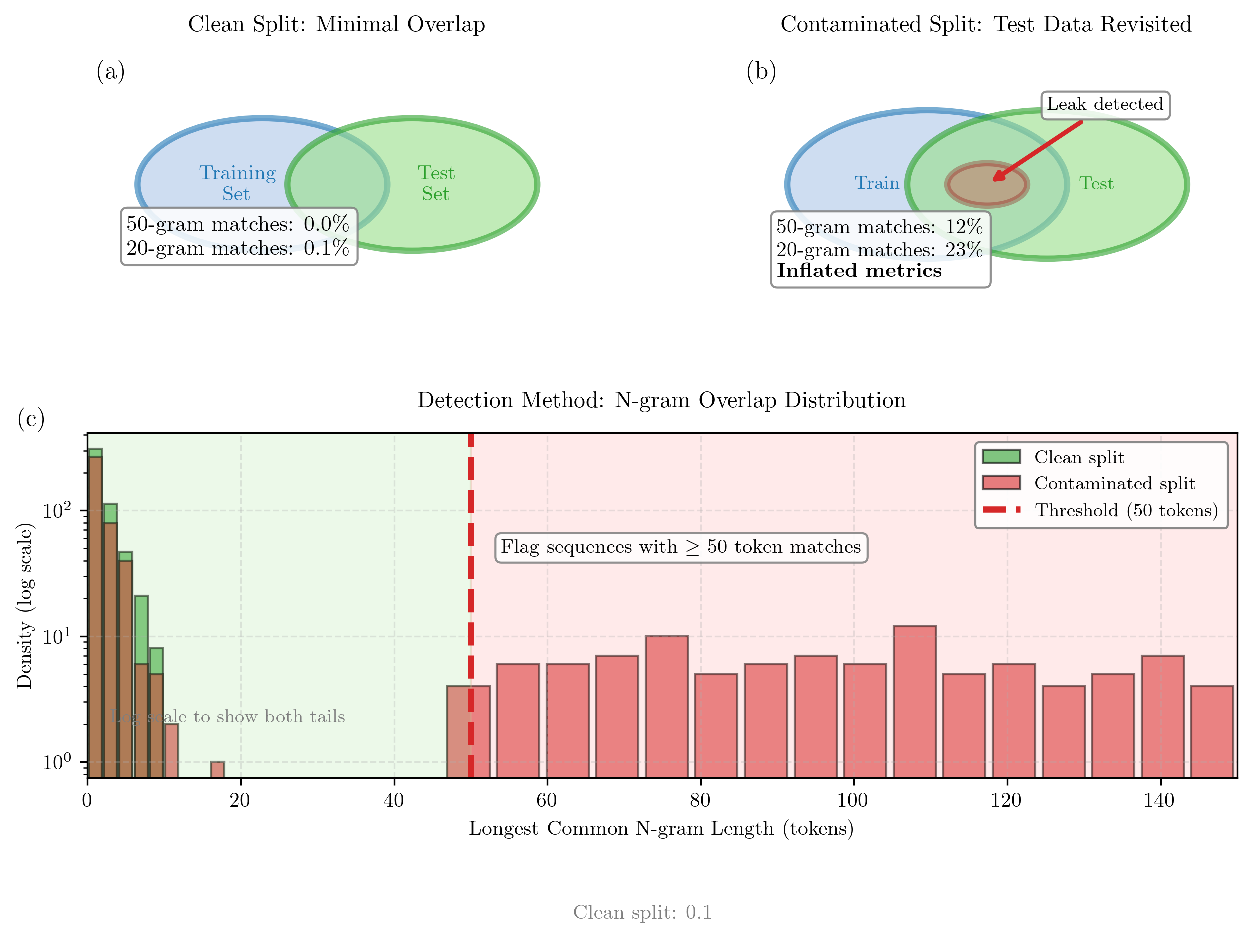
\includegraphics[width=\linewidth]{code/figures/ch10_calibration/fig_10_8_contamination_detection.pdf}
\caption{Contamination checks: deduplicate splits, detect benchmark overlap, and monitor temporal leakage before trusting evaluation results.}
\label{fig:contamination_detection}
\end{figure}

\vspace{0.3cm}

Contamination awareness is about being paranoid in the right way. Assume that any data the model has seen, even indirectly, can inflate your metrics. Document exactly what data was used for training, validation, and testing. When in doubt, exclude suspicious examples rather than including them.

\vspace{1em}

\subsection{Small Hold-Out Sanity Checks}

Before you run a large-scale evaluation, run small sanity checks to catch obvious problems. These are quick tests that can save you from embarrassing failures.

\vspace{0.3cm}

\textbf{Memorization check:} Sample a few examples from your training set and check whether the model can reproduce them exactly or nearly exactly. If it can, you might have overfitting or the model might have memorized large parts of the training set. This does not necessarily mean the model is bad---memorization can coexist with generalization---but it is worth knowing.

\vspace{0.3cm}

\textbf{Random baseline:} Implement a trivial baseline (like always predicting the most common class, or sampling uniformly from the vocabulary) and make sure your model beats it. If your model performs at chance level, something is wrong with the training process or the evaluation setup.

\vspace{0.3cm}

\textbf{Distribution checks:} Plot the distribution of predictions on the test set. Check whether it looks similar to the training distribution or wildly different. If the model assigns very low probability to most test examples, you might have distribution shift. If it assigns very high probability to everything, it might be overconfident.

\vspace{0.3cm}

\textbf{Error analysis on a sample:} Manually inspect ten or twenty test examples where the model failed. What kinds of errors is it making? Are they reasonable mistakes (genuine ambiguity in the data) or systematic failures (a category the model never learned)? This qualitative analysis often reveals patterns that aggregate metrics miss.

\vspace{0.3cm}

These sanity checks take minutes to run but can catch major issues early. Make them a routine part of your evaluation workflow, not something you do only when results look suspicious.

\vspace{1em}

\subsection{Clear Task Rubrics for Generative Outputs}

For generative tasks, evaluation is harder because there is often no single correct answer. A translation can be accurate without being identical to the reference. A summary can capture the key points in many different ways. A creative story can be good or bad by subjective criteria. How do you evaluate these outputs fairly?

\vspace{0.3cm}

The answer is to define a clear rubric---a set of criteria that specify what makes an output good. For each criterion, specify how to measure it, either automatically (using a metric) or manually (using human judgment with clear instructions).

\vspace{0.3cm}

For translation, your rubric might include: accuracy (does it convey the same meaning?), fluency (is it grammatical and natural?), and completeness (are all parts of the source translated?). You might measure accuracy with BLEU or chrF (automatic metrics), fluency with a language model perplexity, and completeness with human judgment.

\vspace{0.3cm}

For summarization, your rubric might include: coverage (does it include the key points?), conciseness (is it brief?), and faithfulness (does it only include information from the source?). Coverage and faithfulness are hard to measure automatically, so you might use human annotators with clear instructions: "Mark a summary as covering the key points if it mentions at least three of the five main events in the article."

\vspace{0.3cm}

For creative tasks, your rubric should align with what users actually care about. If you are evaluating story generation, ask users to rate stories on specific dimensions: coherence, interestingness, emotional impact. Aggregate these ratings to get a multidimensional score, rather than trying to compress quality into a single number.

\vspace{0.3cm}

The key is clarity and reproducibility. Another researcher should be able to read your rubric and apply it the same way you did. Ambiguous criteria like "good quality" or "reasonable output" are not rubrics---they are invitations for bias and inconsistency. Make your criteria concrete, measurable, and tied to what actually matters for your task.

\vspace{2em}

%==========================
\section{What to Report}
%==========================

You have trained your model, evaluated it carefully, and now you need to communicate the results. What should you report? The goal is to provide a small, stable set of numbers and visualizations that tell the truth about your model's capabilities and limitations, without overwhelming the reader with every metric you computed.

\vspace{1em}

\subsection{The Core Metrics: Loss and Task Performance}

Every evaluation should report at least two things: the loss on the test set (typically cross-entropy or perplexity for generative models) and the performance on the downstream task you care about (accuracy, F1, BLEU, or whatever metric aligns with your application).

\vspace{0.3cm}

Loss tells you how well the model fits the test distribution. It is the information-theoretic foundation---the average number of bits or nats needed to encode the test data. Reporting loss allows comparison across different model families and training procedures, because it is a universal metric grounded in compression.

\vspace{0.3cm}

Task performance tells you how well the model does on the thing you actually care about. It is the pragmatic measurement---does the model answer questions correctly, translate accurately, generate coherent text? Task performance can diverge from loss (as we saw earlier in this chapter), so you need both.

\vspace{0.3cm}

\begin{figure}[t]
\centering
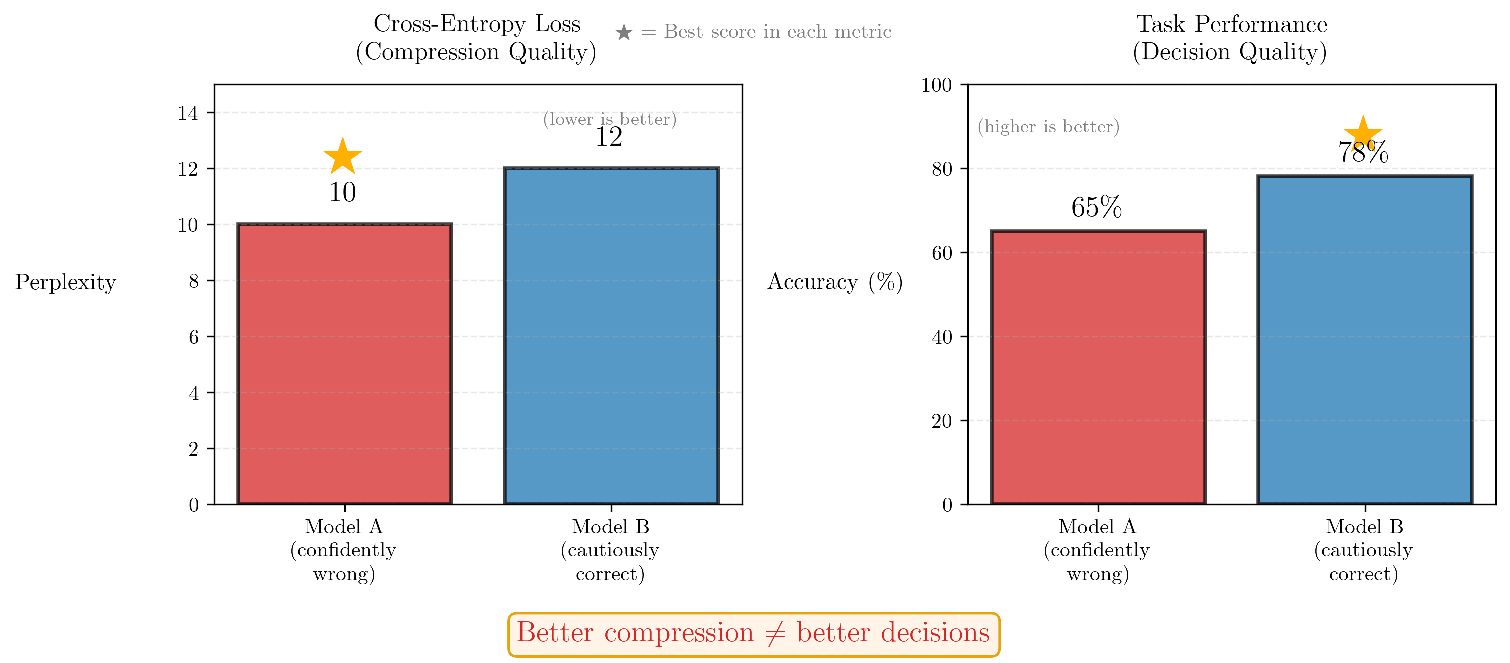
\includegraphics[width=\linewidth]{code/figures/ch10_calibration/fig_10_7_compression_vs_decisions.pdf}
\caption{Lower loss (better compression) does not always imply higher decision performance on downstream tasks; report both to disentangle distribution fit from utility.}
\label{fig:loss_vs_performance}
\end{figure}

\vspace{0.3cm}

For both metrics, report not just the mean but also a measure of uncertainty. If you have multiple test sets, report per-set results. If you have multiple runs with different random seeds, report mean and standard deviation across runs. If you have a single test set and a single run, report bootstrap confidence intervals. Uncertainty quantification turns a point estimate into an honest statement about what you know.

\vspace{1em}

\subsection{Calibration Curves: Trust and Reliability}

If your model outputs probabilities that will be used for decision-making, you must report calibration. The simplest way to do this is to include a reliability diagram in your evaluation report. This single plot communicates whether the model's confidence is trustworthy.

\vspace{0.3cm}

Alongside the plot, report a calibration metric. Expected Calibration Error (ECE) is the most common: you bin predictions by confidence, compute the difference between average confidence and actual accuracy in each bin, and take the weighted average of these differences across bins. Lower ECE means better calibration. ECE is simple, but it depends on how you define confidence and how you choose bins, so report those choices alongside the number.

\vspace{0.3cm}

If you applied post-hoc calibration (like temperature scaling), report both the uncalibrated and calibrated ECE. This shows whether calibration was necessary and whether your calibration method worked. Also report the temperature value or calibration parameters, so others can reproduce your calibration procedure.

\vspace{0.3cm}

For generative models, token-level and sequence-level calibration might both matter. If so, report both, with clear explanations of what each measures. Token-level calibration can be computed on every token prediction in your test set. Sequence-level calibration requires aggregating across full sequences and might involve human evaluation to define "quality," so it is harder to compute, but it is often more relevant for deployment.

\vspace{1em}

\subsection{Sample Outputs: The Qualitative Evidence}

Numbers are essential, but they do not tell the whole story. Sample outputs give readers a qualitative sense of what the model actually does. Include a diverse set of examples: good ones that showcase the model's strengths, bad ones that reveal its weaknesses, and edge cases that illustrate failure modes.

\vspace{0.3cm}

For each sample, provide context: what was the input, what did the model generate, and why is this example notable? If you are comparing multiple models, show outputs from each model on the same input, so readers can see the differences directly.

\vspace{0.3cm}

Resist the temptation to cherry-pick only impressive examples. This is dishonest evaluation. Include failures. Show where the model hallucinates, contradicts itself, or produces nonsense. These examples are as informative as the successes, because they reveal the model's limitations and where it should not be trusted.

\vspace{0.3cm}

For generative models with high variance (where the same input can produce many different outputs), show multiple samples from the same input. This illustrates the diversity and consistency of the model. If the model produces ten very similar outputs, it is deterministic. If it produces ten wildly different outputs, it is exploring the space broadly, which might be good or bad depending on your task.

\vspace{1em}

\subsection{Ablations and Comparisons: Understanding What Matters}

To understand why your model works, include ablation studies: experiments where you remove or change one component and measure the effect on performance. Did the extra training data help? Did the architectural change improve results? Did the specific hyperparameter choice matter?

\vspace{0.3cm}

Ablations turn a single result into a scientific understanding. They tell you which design decisions were critical and which were incidental. They also help future work build on your results, because they identify the key ingredients rather than just reporting the final recipe.

\vspace{0.3cm}

Comparisons to baselines and prior work are equally important. You should include at least three reference points: a simple baseline (to show the task is not trivial), the previous state of the art (to show your improvement), and a well-tuned standard approach (to show your method's advantage over reasonable alternatives). Each comparison answers a different question about your model's contribution.

\vspace{0.3cm}

When reporting comparisons, be fair. Use the same evaluation protocol for all models. If you tuned hyperparameters for your model, tune them for baselines too. If you used data augmentation, apply it to baselines as well. Unfair comparisons are uninformative at best and misleading at worst.

\vspace{1em}

\subsection{What Not to Report}

Finally, here is what you should \emph{not} report, or at least not prominently: metrics that do not measure what you care about. Every number you include should serve a purpose. If a metric does not inform a decision or answer a question, it is clutter.

\vspace{0.3cm}

Avoid reporting dozens of metrics on dozens of benchmarks just to fill a table. This creates information overload and obscures the key findings. Pick the three to five most relevant metrics, explain why they matter, and report those clearly. If you computed other metrics during development, mention them briefly or move them to an appendix, but do not let them dominate the narrative.

\vspace{0.3cm}

Avoid reporting metrics that are not calibrated to task importance. If your task has rare but critical failures, accuracy might look great while the model is actually dangerous. Report precision and recall, or better yet, define a task-specific cost function that weights different errors appropriately.

\vspace{0.3cm}

Avoid using metrics just because they are standard. If BLEU does not correlate with translation quality for your model and task, do not report it as your primary metric. Use human evaluation or a metric that actually measures what you care about. Following convention is valuable for comparability, but not when the convention measures the wrong thing.

\vspace{2em}

%==========================

\begin{pausebox}
\textbf{Pause and Reflect}

\vspace{0.3cm}

Before moving on, take a moment to consolidate. Can you explain why cross-entropy measures average codelength and what this tells you about a model? Can you describe the difference between a well-calibrated and a poorly calibrated model, and why calibration matters for decisions? Can you articulate the tradeoff between temperature, diversity, and error rate in sampling? Can you list three types of contamination that invalidate evaluation and how to detect them? Can you explain what metrics you would report for a generative model and why each one matters?

\vspace{0.3cm}

If any of these feel unclear, revisit the relevant section. Evaluation is where theory meets practice---where the information-theoretic foundations we have built throughout this book translate into concrete measurements that guide real decisions. The discipline of honest evaluation, more than any single technique, separates systems that work from systems that merely pass tests.
\end{pausebox}

\vspace{1em}

This chapter has equipped you with the essential tools for evaluating generative models honestly. We began by understanding what evaluation really measures: cross-entropy and perplexity quantify average codelength, but they do not tell you whether the model's uncertainties are trustworthy or whether it makes good decisions. We explored calibration, the alignment between confidence and correctness, and learned simple techniques like temperature scaling to fix calibration failures. We examined sampling strategies---temperature, top-$k$, and nucleus sampling---and understood how each controls the tradeoff between diversity and error rate. We established practical protocols for clean evaluation: guard against contamination, run sanity checks, and define clear rubrics for generative tasks. And we distilled what to report: a small set of metrics grounded in information theory and task performance, supplemented by sample outputs, ablations, and honest acknowledgment of failures.

\vspace{0.3cm}

Evaluation is honest bookkeeping. The numbers you report are statements about how efficiently your model encodes information, how reliably it quantifies uncertainty, and how well it performs the task you care about. This chapter has given you the framework to make those statements truthfully.

\vspace{0.3cm}

In the next chapter, we will turn to a different challenge: how to build systems that use generative models as components in larger workflows. We will explore prompting strategies, tool use, retrieval augmentation, and other techniques that extend a model's capabilities beyond what it learned during training. The evaluation principles from this chapter will guide us: we will measure not just the model's performance in isolation, but the performance of the full system in realistic deployment scenarios. The information-theoretic foundation remains the same---learning is compression, and good systems compress efficiently---but the engineering challenges multiply when models interact with external knowledge, tools, and human feedback.
